\documentclass{article}

% Font
\usepackage[T1]{fontenc}
\usepackage[utf8]{inputenc}
\usepackage{lmodern}

% For tables
\usepackage{multirow}

% For identing the table at the right place
\usepackage{float}

% For left spacing
\usepackage{scrextend}

% For images
\usepackage{graphicx}

% for shorter paragraph spaces
\setlength{\parindent}{1ex}
\setlength{\parskip}{0.5ex}
% for first paragraphs
\newcommand*\fpar{\hspace{1ex}}

\title{Project 1 Requirements}
\author{Group 14 \\
Tiago Carvalho fc51034 \\
Diogo Lopes fc51058 \\
João Roque fc51080 \\
Miguel Saldanha fc51072 \\
João Afonso fc51111 \\
}
\date{21/04/2021}

\begin{document}
\maketitle

\section{Use Cases}
  \begin{table}[H]
    \centering
    \begin{tabular}{c|c|l} 
      Services & User & Functionalities \\ \hline
      \multirow{7}{*}{ Normal }
        & \multirow{5}{*}{ Regular } 
          & User Log in/Sign in \\
        & & See Book, Show and Movie Library \\
        & & Set Book/Show/Movie as seen \\
        & & Set Book/Show/Movie as liked \\ 
        & & Ask for suggestions to read and/or watch \\ \cline{2-3}
      & \multirow{2}{*}{ Admin } 
          & Add Book/Show/Movie to Library \\
        & & Remove Book/Show/Movie from Library \\ \hline
      \multirow{2}{*}{ Spark }
        & \multirow{2}{*}{ Regular }
          & Count how many views a specific Item has \\
        & & Count how many likes a specific Item has \\
    \end{tabular}
  \end{table}

\section{Preliminary Functional and Non-Functional Requirements}
\textbf{SPARK note}: Since our likes and views are stored inside each User, Spark makes sense in this context because we need to go through every single one of them to calculate it. A different approach would be storing views and likes in the Item itself, but for this implementation suits well our needs.
  
  \subsection{Functional}
    \begin{itemize}
      \item User should be able to browse Books, Shows and Movies.
      \item User should be able to search for a specific item by name, type and/or categories.
      \item User should be able to mark an Item as seen.
      \item User should be able to mark an Item as liked.
      \item User should be able to ask for suggestions.
      \item Admin should be able to add and remove content from the library.
      \item \textbf{(Spark)} User should be able to see how many likes and views a specific Item has.
    \end{itemize}

  \subsection{Non-Functional}
    \begin{itemize}
      \item Browsing Items shouldn't take more than $1.5$ seconds to load.
      \item Searching shouldn't take more than $2.5$ seconds loading the response.
      \item Marking Item as seen or liked shouldn't take loading time on Users' end.
      \item Suggestions shouldn't take more than $5$ seconds.
      \item Data stored in cache shouldn't affect the system.
      \item Adding and Removing Items should persist on the database.
      \item \textbf{(Spark)} Calculating views and like from an Item shouldn't take more than $1$ second.
    \end{itemize}

\section{Preliminary Architectural Design}
  \begin{figure}[H]
    \centering
    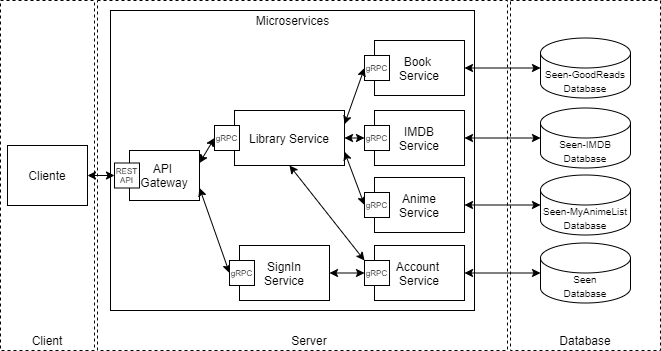
\includegraphics[width=\textwidth]{"images/CloudNativeAppArchitecture.png"}
  \end{figure}

\end{document}